\section{Qualitative Analysis\label{sec:sota.quali}}

This section contains the results of our literature review.
First, it synthesizes the analyses into a reference architecture and a taxonomy for \glspl{fids}, which help structure the field.
Then, it goes over a comparison of the selected works to answer \Cref{rq:sota.components,rq:sota.metrics,rq:sota.techniques} on the components of \glspl{fids} and their impact on performance.


\subsection{Structuring the Literature\label{sec:sota.quali.structure}}

The qualitative (\Cref{sec:sota.quali}) and quantitative (\Cref{sec:sota.quanti}) analyzes provide results that we synthesize hereafter in a reference architecture and a taxonomy.
The reference architecture presents the components of \glspl{fids} and their interactions, while the taxonomy provides comparison criteria for the selected works.

We build the taxonomy upon different existing ones related to \gls{cids}
\cite{vasilomanolakis_TaxonomySurveyCollaborative_2015,zhou_surveycoordinatedattacks_2010}, \gls{ml}--based intrusion detection~\cite{dacosta_InternetThingssurvey_2019}, and
\gls{fl} \cite{aledhari_FederatedLearningSurvey_2020,lyu_ThreatsFederatedLearning_2020,mothukuri_surveysecurityprivacy_2021}.
First, we extract classes relevant to the domain
of \gls{fids}, before filtering out irrelevant ones by validating the taxonomy against the reference architecture (\Cref{fig:sota.archi}).
The latter displays both the operation and
the design of the system.
By confronting the taxonomy and the architecture, we ensure that each item
of the taxonomy is related to a component of the architecture, and \emph{vice versa}.
Then, we add any commonalities between the selected works that are not already represented in the previous taxonomies.
This identifies new criteria on which to compare the selected works.


\subsubsection{Reference Architecture\label{sec:sota.discuss.synthesis.archi}}

\begin{figure*}
  \centering
  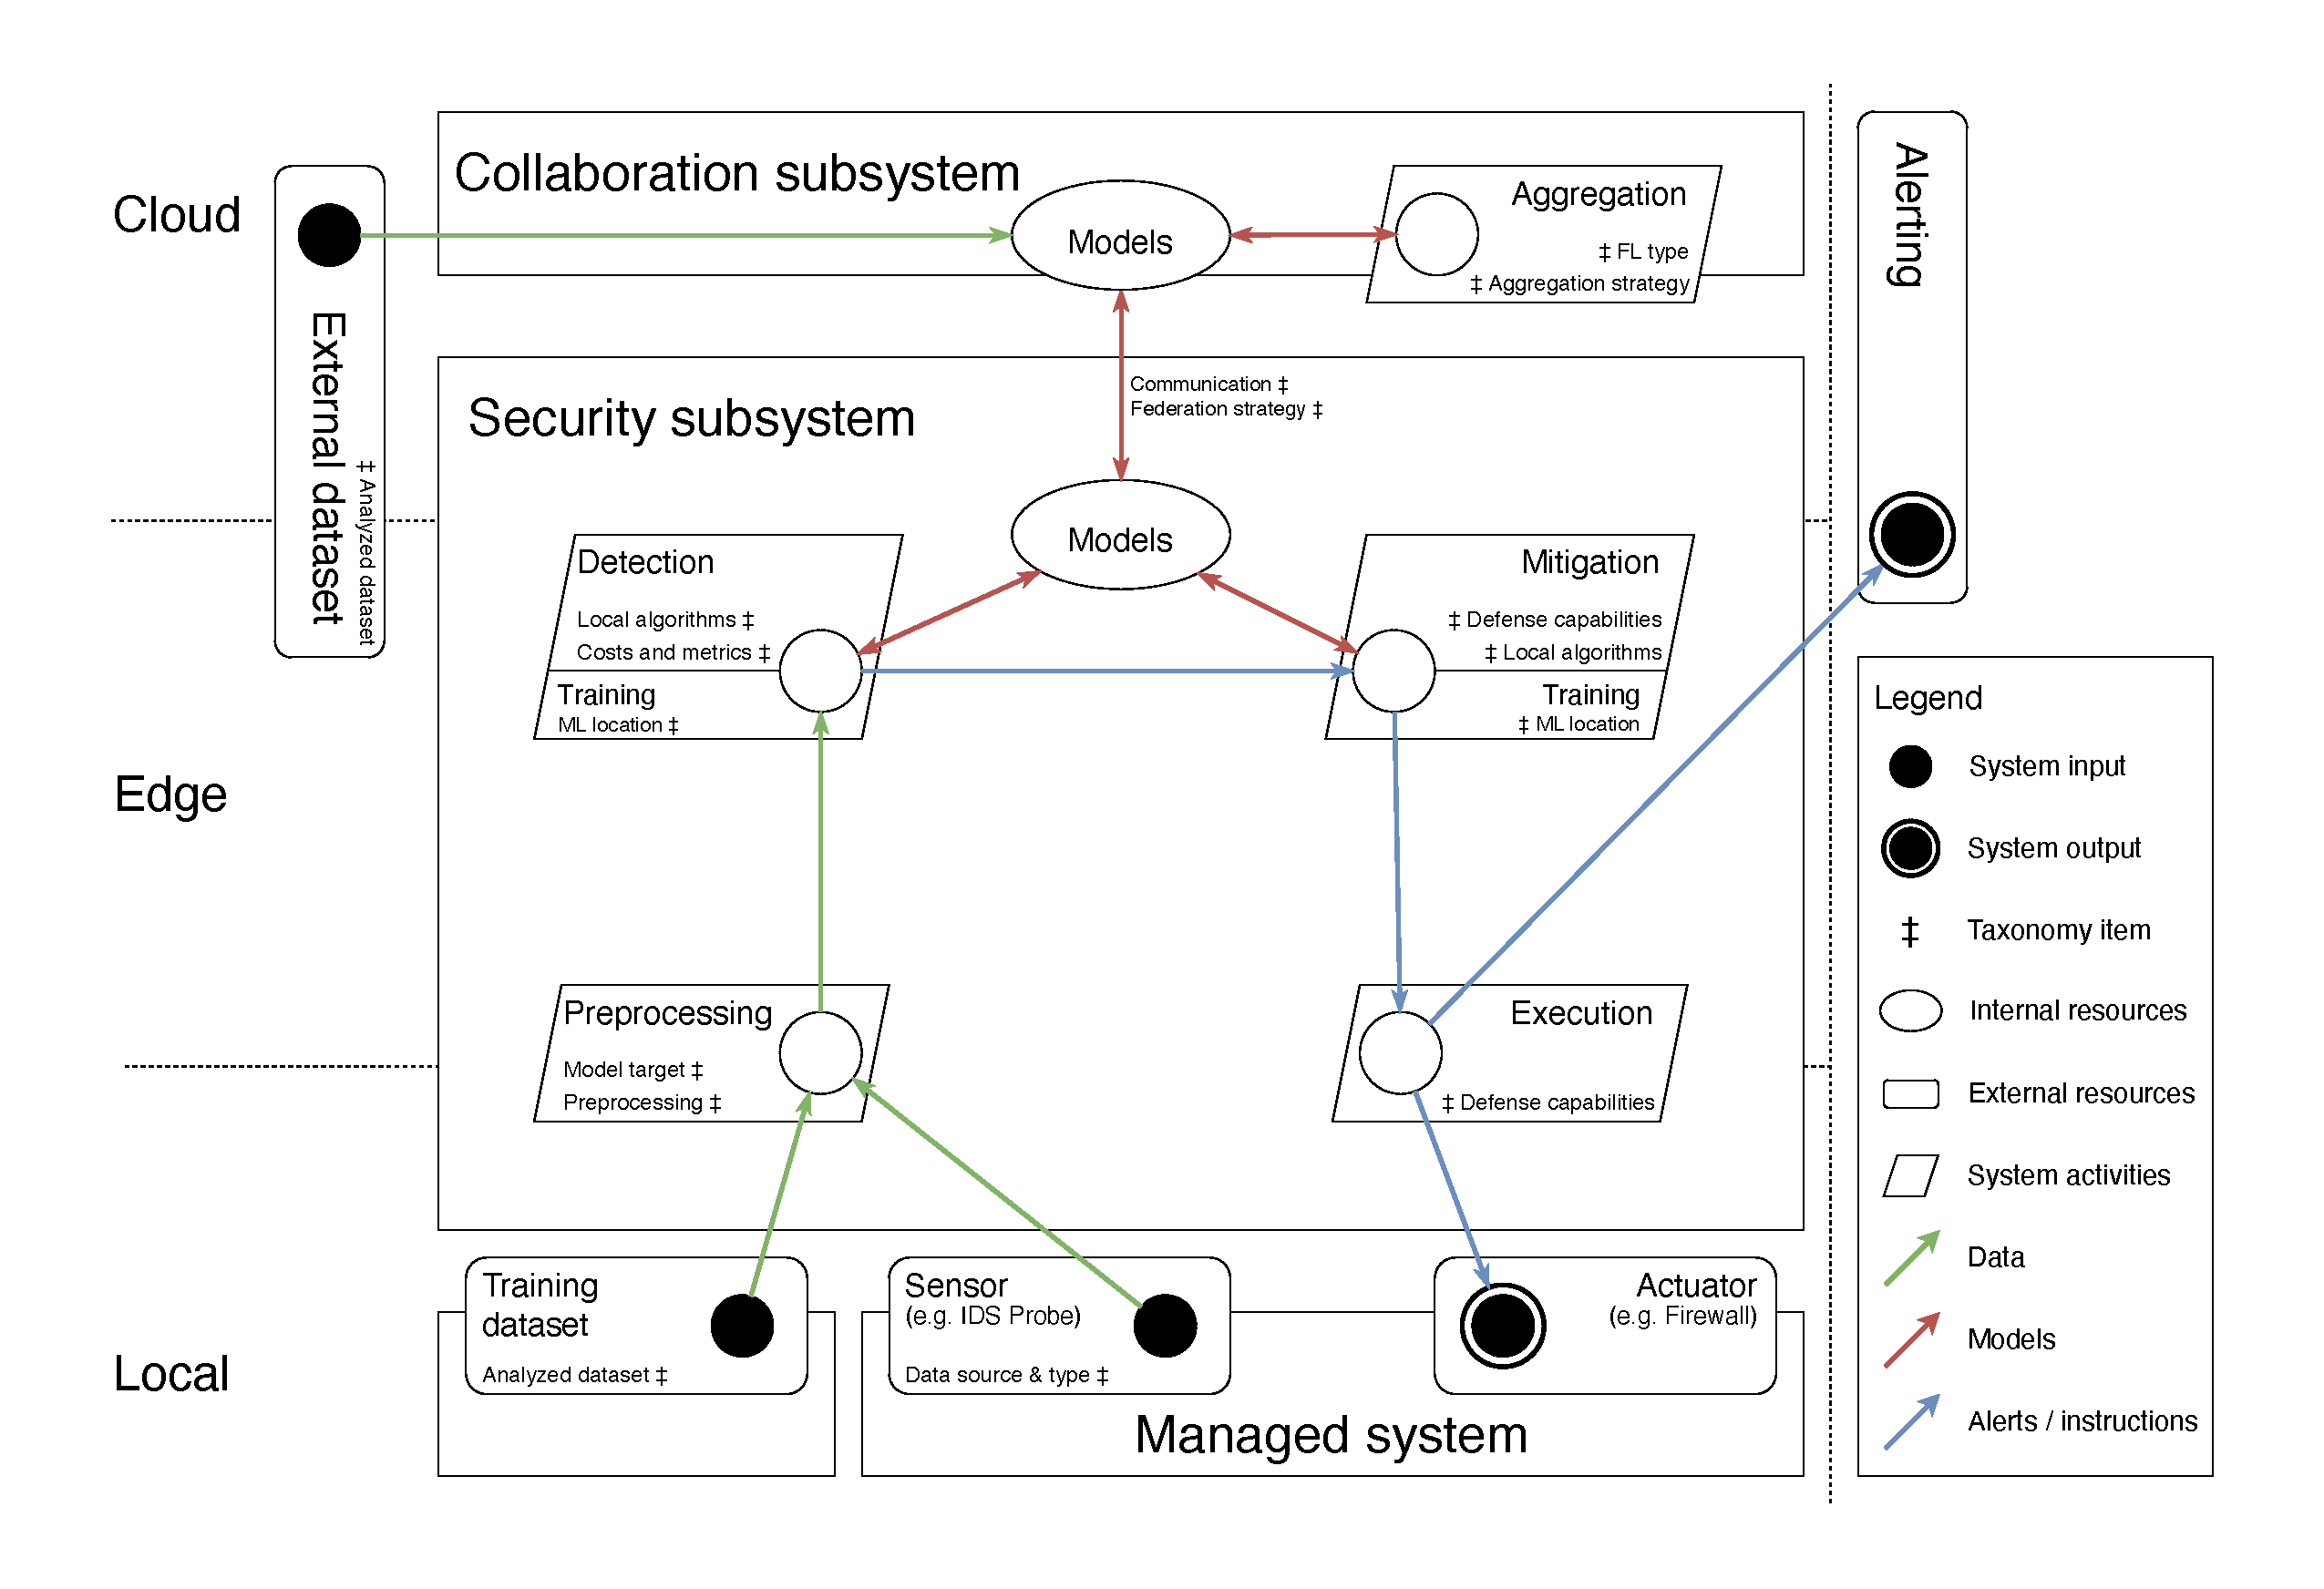
\includegraphics[width=.95\textwidth]{figures/architecture.drawio.pdf}
  \caption[
    The proposed reference architecture for \glspl{fids}.
  ]{
    The proposed reference architecture for \glspl{fids}.
    Figure from \textcite{lavaur_EvolutionFederatedLearningbased_2022} \copyright~IEEE 2022.
    \label{fig:sota.archi}
  }
\end{figure*}

This section presents the reference architecture synthesized from the selected works, as depicted in \Cref{fig:sota.archi}.
The architecture provides a summary of the components of \glspl{fids} and their interactions, answering \Cref{rq:sota.components}.
It can be divided in three parts:
\begin{itemize}
  \item The \emph{Managed system} represents the monitored system, \eg, \gls{it} network, industrial devices, or health-monitoring wearables.
  As noticed in \Cref{sec:sota.quali.data}, collected data can either concern system or environment behavior.
  The former relates to information generated by the systems, \eg, network traces or resource consumption.
  The latter refers to what the monitored system operates on, \eg, health metrics for medical devices of temperature and atmospheric pressure for building management systems.
  
  \item The \emph{Security subsystem} is the core of the architecture.
  It contains all the system's activities, from model training to detection and counter-measures deployment.
  Depending on the objectives and constraints, this subsystem can either be run locally like \cite{pahl_AllEyesYou_2018} or \cite{hei_trustedfeatureaggregator_2020}, on a dedicated edge-device as in \cite{li_DeepFedFederatedDeep_2020}.
  In the case of centralized learning, this entire subsystem runs in the cloud.
  The subsystem is assumed to run a device that embeds enough computing power to perform real-time anomaly detection against \gls{ml} models.
  It is also capable of training its own model based on collected data.

  \item The \emph{Collaboration subsystem} provides the \emph{sharing} feature of the system, essentially model aggregation (\Cref{sec:sota.quali.agg}).
  It also provides optional training from other sources, like online datasets.
\end{itemize}

This architecture has similarities with the principles of autonomic systems, as defined by IBM in 2001~\cite{kephart_visionautonomiccomputing_2003}, referred to as \gls{mape-k}.
Classic autonomic systems are local, and therefore use a database to provide \emph{knowledge}.
In \gls{fids}, \gls{fl} fills this role in the reference architecture, as the knowledge is being shared among all agents through model aggregation.


\subsubsection{Taxonomy for FIDS\label{sec:sota.discuss.synthesis.taxo}}

The taxonomy depicted in \Cref{fig:sota.taxonomy} summaries the core components and specificities of \glspl{fids}, as extracted from the selected works and existing related taxonomies.
Correlations between the taxonomy items and the system's components can be seen in the reference architecture (\Cref{fig:sota.archi}).
It also serves as a framework for the comparisons of the selected works.
Each class represents a building block, for which multiple approaches exist depending on use case and constraints.

\begin{figure}
  \centering
  \resizebox{\textwidth}{!}{

\usetikzlibrary{trees,positioning,shapes,shadows,arrows,arrows.meta,angles,quotes}

\definecolor{yellowfill}{HTML}{FFF2CC}
\definecolor{yellowstroke}{HTML}{D6B656}

\definecolor{grayfill}{HTML}{F5F5F5}
\definecolor{graystroke}{HTML}{666666}

\forestset{
  forked edge'/.style={
    edge={rotate/.option=!parent.grow},
    edge path'={
      (.child anchor)
      -- ++(-\forestoption{fork sep},0)
      |- (!u.parent anchor)
    },
  },
}

\newcommand{\lkbx}[1]{\mbox{#1\strut}}



        \begin{forest}
        forked edges,
        for tree={
            rounded corners,
            grow=east,
            inner ysep=1.2ex, 
            anchor=base west,
            l sep+=3em,
            fork sep=2.5em,
            tier/.option=level,
            where level=0{%
                draw,
                draw=yellowstroke,
                fill=yellowfill,
                inner sep=4ex,
                font=\Large\bfseries,
            }{},
            where level=1{%
                draw,
                draw=graystroke,
                fill=grayfill,
                inner sep=3ex,
                font=\Large,
            }{},
            where level=2{%
                draw,
                draw=graystroke,
                fill=grayfill,
                inner sep=3ex,
                font=\large,
            }{},
        },
        parent anchor=east,
        [{Taxonomy of FIDS}
            [Experimentation
                [12. \lkbx{\fullcref{sec:sota.quali.metrics}}
                    [Execution
                        [Performance (\eg accuracy)]
                        [Latency]
                    ]
                    [Federation
                        [Communication]
                        [Aggregation]
                    ]
                    [Training
                        [Resources (\eg hardware)]
                        [Time (\eg convergence)]
                    ]
                ]
                [11. \lkbx{\fullcref{sec:sota.quali.dataset}}
                    [Public / Known]
                    [Published but custom]
                    [Unpublished (as of now)]
                ]
            ]
            [Aggregation
                [10. \lkbx{\fullcref{sec:sota.quali.target}}
                    [By-device]
                    [Personalized model
                        [By-class]
                        [By performance]                
                    ]
                    [Generic model]
                ]
                [9. \lkbx{\fullcref{sec:sota.quali.agg}}
                    [Parameter aggregation (\eg FedAvg)]
                    [Weighted algorithms]
                    [MPC-based aggregation]
                ]
                [8. \lkbx{\fullcref{sec:sota.quali.type}}
                    [Horizontal Federated Learning]
                    [Vertical Federated Learning]
                    [Federated Transfer Learning]
                ]
            ]
            [Federation
                [7. \lkbx{\fullcref{sec:sota.quali.comm}}
                    [Encryption]
                    [Overhead reduction]
                ]
                [6. \lkbx{\fullcref{sec:sota.quali.fed}}
                    [Client selection]
                    [Reputation]
                    [Architecture (\eg P2P)]
                ]
            ]
            [Local operation
                [5. \lkbx{\fullcref{sec:sota.quali.defense}}
                    [Network reconfiguration (\eg SDN)]
                    [On-device counter-measures]
                ]
                [4. \lkbx{\fullcref{sec:sota.quali.alg}}
                    [Supervised ML
                        [Classification]
                        [Regression]
                    ]
                    [Unsupervised ML
                        [Clustering]
                        [Dimensionality reduction]
                        [Outlier detection]
                    ]
                    % [Detection method
                    %     [Anomaly-based]
                    %     [Signature-based]
                    %     [Specification-based]
                    %     [Hybrid]
                    % ]
                ]
                [3. \lkbx{\fullcref{sec:sota.quali.location}}
                    [On device]
                    [On gateway]
                    [Dedicated device]
                    [On server]
                ]
            ]
            [Data
                [2. \lkbx{\fullcref{sec:sota.quali.preprocess}}
                    [Feature selection]
                    [Feature extraction]
                    [Dimensionality reduction]
                ]
                [1. \lkbx{\fullcref{sec:sota.quali.data}}
                    [Source
                        [Communication]
                        [Usage]
                    ]
                    [Distribution
                        [IID]
                        [Non-IID]
                    ]
                ]
            ]
        ]
    \end{forest}
}
  \caption[
    Proposed taxonomy for FIDS.
  ]{
   \emph{Proposed taxonomy for FIDS.}
    Figure from \textcite{lavaur_EvolutionFederatedLearningbased_2022} \copyright~IEEE 2022.
    \label{fig:sota.taxonomy}
  }
\end{figure}


The proposed taxonomy contains 12 classes describing the selected works that span over five main aspects:
\begin{itemize}
  \item Two classes cover the topic of \textbf{Data}: \emph{\nameref*{sec:sota.quali.data}} and \emph{\nameref*{sec:sota.quali.preprocess}}.
  It defines the type of data considered and how it is distributed among clients, how it is collected, and the preprocessing strategies that are used.
  
  \item \textbf{Local operation} is represented by 3 classes: \emph{\nameref*{sec:sota.quali.location}}, \emph{\nameref*{sec:sota.quali.alg}}, and \emph{\nameref*{sec:sota.quali.defense}}.
  It describes the detection and mitigation strategies, how models are built and trained, and where the computing resources are located.
  
  \item The \textbf{Federation} aspect is covered by 2 classes: \emph{\nameref*{sec:sota.quali.fed}} and \emph{\nameref*{sec:sota.quali.comm}}.
  They refer to the communication between the agents and the server, and how data sharing is organized.
  
  \item \textbf{Aggregation} is also covered by 3 classes: \emph{\nameref*{sec:sota.quali.type}}, \emph{\nameref*{sec:sota.quali.agg}}, and \emph{\nameref*{sec:sota.quali.target}}.
  It describes the type of \gls{fl} used, how the models are merged, in accordance with the objectives of the system.
  
  \item Finally, 2 classes address the \textbf{Experimentation} topic: \emph{\nameref*{sec:sota.quali.dataset}} and \emph{\nameref*{sec:sota.quali.metrics}}.
  This meta-category does not relate to the proposed solution, but to how the experiments are performed.
\end{itemize}



\subsection{Federated Learning for Intrusion Detection\label{sec:sota.quali.fids}}

This section reviews the selected literature.
Using the taxonomy as a reference, it details and compares the selected works.
\Cref{tbl:sota.comp} summarizes the information and helps identify differences between the works.
It gives partial answers to research questions about the components of \glspl{fids} and how to measure their impact on performance (\Cref{rq:sota.components,rq:sota.metrics}), while \Cref{sec:sota.quali.agg} replies to \Cref{rq:sota.techniques} about federation techniques.


\begin{table}
  \centering
  \caption{
    Comparative overview of selected works in the original study---approach and objectives (1/2).%
    \label{tbl:sota.comp}%
  }%
  \resizebox{\textwidth}{!}{% LTeX: enabled=false
        
\newcommand*\rotbr[1]{\hbox to1.5em{\hss\rotatebox[origin=br]{-50}{#1}}}
\newcommand*\rotbl[1]{\hbox to1.5em{\hss\rotatebox[origin=tl]{50}{#1}}} % kept to rotate the bottom row if needed
\newcommand*\rotl[1]{\hbox to1em{\hss\rotatebox{90}{#1}}}
\newcommand*\rotb[1]{#1}
\newcommand*\yes{\CIRCLE}
\newcommand*\partly{\LEFTcircle}
\newcommand*\nop{\Circle}

%\renewcommand{\arraystretch}{2} % add vertical space
% define a tabular environment that has an arraystretch value of 1, allowing
% the main table to have another value.
\newenvironment{1xtabular}[1][1]{%
    \renewcommand*{\arraystretch}{1}%
    \tabular%
}{%
    \endtabular
}

\newenvironment{2xtabular}[1][1]{%
    \renewcommand*{\arraystretch}{2.5}%
    \tabular%
}{%
    \endtabular%
}

\newcommand{\wcell}[1]{\begin{1xtabular}[c]{@{}l@{}}#1\end{1xtabular}}

\begin{threeparttable}

    % WHEN PASTING THE TABLE FROM TABLEGENERATOR:
    % - add the @{} when needed to collapse columns 
    % - replace the in-table tabular environment by `1tabular`
    \begin{2xtabular}{@{}llc@{}c@{}c@{}c@{}cc@{}c@{}c@{}c@{}cc@{}c@{}c@{}c@{}cc@{}clll@{}}
        \toprule
        \multicolumn{1}{c}{} & \multicolumn{1}{c}{Ref}                                                          & \rotbr{Internet of Things} & \rotbr{Information Technologies} & \rotbr{Cyber Physical Systems} & \rotbr{Autonomous Vehicles} & \rotbr{Satellite-terrestrial networks} & \rotbr{Horizontal FL} & \rotbr{Vertical FL} & \rotbr{Federated Transfer Learning} & \rotbr{Federated MTL} & \rotbr{Federated Mimic Learning} & \rotbr{Online learning} & \rotbr{Supervised}  & \rotbr{Semi-supervised}   & \rotbr{Unsupervised}  & \rotbr{Personalized models} & \rotbr{Network-based} & \rotbr{Usage-based} & \multicolumn{1}{c}{Training location}       & \multicolumn{1}{c}{Data type}                         & \multicolumn{1}{c}{Strengths}                                                      \\ \midrule   
        2018                 & \mbox{\textcite{pahl_AllEyesYou_2018}\strut}                                     & \yes                       & \nop                             & \nop                           & \nop                        & \nop                                   & \yes                  & \nop                & \nop                                & \nop                  & \nop                             & \yes                    & \nop                & \nop                      & \yes                  & \yes                        & \yes                  & \nop                & Device                                      & \wcell{Abstracted network\\ traffic (middleware)}     & \wcell{relatively lightweight,\\ online, no labels}                                \\            
        2019                 & \mbox{\textcite{rathore_BlockSecIoTNetBlockchainbaseddecentralized_2019}\strut}  & \nop                       & \yes                             & \nop                           & \nop                        & \nop                                   & \yes                  & \nop                & \nop                                & \nop                  & \nop                             & \nop                    & \yes                & \nop                      & \nop                  & \yes                        & \yes                  & \nop                & \wcell{Edge-controller\\ (SDN)}             & Network traffic (SDN)                                 & \wcell{offers mitigation,\\ decentralized}                                         \\            
        2019                 & \mbox{\textcite{schneble_Attackdetectionusing_2019}\strut}                       & \yes                       & \nop                             & \nop                           & \nop                        & \nop                                   & \yes                  & \nop                & \nop                                & \nop                  & \nop                             & \yes                    & \nop                & \nop                      & \yes                  & \yes                        & \yes                  & \nop                & Gateway                                     & \wcell{IoT network\\ traffic (TCPdump)}               & \wcell{online, offers per-class\\ models, no labels}                               \\            
        2019                 & \mbox{\textcite{nguyen_DIoTFederatedSelflearning_2019}\strut}                    & \nop                       & \yes                             & \nop                           & \nop                        & \nop                                   & \nop                  & \nop                & \nop                                & \yes                  & \nop                             & \nop                    & \yes                & \nop                      & \nop                  & \yes                        & \yes                  & \nop                & Gateway                                     & \wcell{Encrypted network\\ traffic (CICFlowMeter)}    & versatile (multi-task)                                                             \\            
        2019                 & \mbox{\textcite{zhao_MultiTaskNetworkAnomaly_2019}\strut}                        & \nop                       & \nop                             & \yes                           & \nop                        & \nop                                   & \yes                  & \nop                & \nop                                & \nop                  & \nop                             & \yes                    & \nop                & \nop                      & \yes                  & \nop                        & \nop                  & \yes                & Gateway                                     & Healthcare sensor values                              & high adaptability, no labels                                                       \\            
        2019                 & \mbox{\textcite{cetin_FederatedWirelessNetwork_2019}\strut}                      & \nop                       & \yes                             & \nop                           & \nop                        & \nop                                   & \yes                  & \nop                & \nop                                & \nop                  & \nop                             & \nop                    & \yes                & \nop                      & \nop                  & \nop                        & \yes                  & \nop                & Gateway                                     & Network traffic (WIFI)                                & --                                                                                 \\            
        2020                 & \mbox{\textcite{li_DeepFedFederatedDeep_2020}\strut}                             & \yes                       & \nop                             & \nop                           & \nop                        & \nop                                   & \yes                  & \nop                & \nop                                & \nop                  & \nop                             & \nop                    & \yes                & \nop                      & \nop                  & \nop                        & \nop                  & \yes                & Gateway                                     & \wcell{Air conditioner\\ sensor values}               & offers traceability (blockchain)                                                   \\            
        2020                 & \mbox{\textcite{chen_Networkanomalydetection_2020}\strut}                        & \nop                       & \nop                             & \yes                           & \nop                        & \nop                                   & \yes                  & \nop                & \nop                                & \nop                  & \nop                             & \nop                    & \yes                & \nop                      & \nop                  & \nop                        & \yes                  & \nop                & Gateway                                     & MODBUS traffic                                        & confidentiality (encryption)                                                       \\            
        2020                 & \mbox{\textcite{zhang_BlockchainbasedFederatedLearning_2020}\strut}              & \nop                       & \yes                             & \nop                           & \nop                        & \nop                                   & \yes                  & \nop                & \nop                                & \nop                  & \nop                             & \nop                    & \yes                & \nop                      & \nop                  & \nop                        & \yes                  & \nop                & Device                                      & \wcell{IoT network\\ traffic (TCPdump)}               & --                                                                                 \\            
        2020                 & \mbox{\textcite{fan_IoTDefenderFederatedTransfer_2020}\strut}                    & \nop                       & \yes                             & \nop                           & \nop                        & \nop                                   & \yes                  & \nop                & \nop                                & \nop                  & \nop                             & \nop                    & \nop                & \nop                      & \yes                  & \nop                        & \yes                  & \nop                & Gateway                                     & \wcell{IoT network\\ traffic (TCPdump)}               & no labels                                                                          \\            
        2020                 & \mbox{\textcite{rahman_InternetThingsIntrusion_2020}\strut}                      & \nop                       & \yes                             & \nop                           & \nop                        & \nop                                   & \yes                  & \nop                & \nop                                & \nop                  & \nop                             & \nop                    & \yes                & \nop                      & \nop                  & \yes                        & \yes                  & \nop                & Gateway                                     & \wcell{Network traffic\\ (PCAP)}                      & \wcell{segmented (performance-\\based models)}                                     \\            
        2020                 & \mbox{\textcite{sun_IntrusionDetectionSegmented_2020}\strut}                     & \yes                       & \nop                             & \nop                           & \nop                        & \nop                                   & \nop                  & \nop                & \yes                                & \nop                  & \nop                             & \nop                    & \yes                & \nop                      & \nop                  & \yes                        & \yes                  & \nop                & \wcell{Gateway\\ (MEC)}                     & \wcell{IoT network traffic\\ (TCPdump, CICFlowMeter)} & \wcell{knowledge transfer between\\ public and private datasets}                   \\            
        2020                 & \mbox{\textcite{al-athbaal-marri_FederatedMimicLearning_2020}\strut}             & \nop                       & \yes                             & \nop                           & \nop                        & \nop                                   & \nop                  & \nop                & \nop                                & \nop                  & \yes                             & \nop                    & \yes                & \nop                      & \nop                  & \nop                        & \yes                  & \nop                & Gateway                                     & \wcell{Network traffic\\ (TCPdump)}                   & \wcell{enhanced privacy\\ (mimic learning)}                                        \\            
        2020                 & \mbox{\textcite{kim_CollaborativeAnomalyDetection_2020}\strut}                   & \nop                       & \yes                             & \nop                           & \nop                        & \nop                                   & \yes                  & \nop                & \nop                                & \nop                  & \nop                             & \nop                    & \yes                & \nop                      & \nop                  & \nop                        & \yes                  & \nop                & Gateway                                     & \wcell{Network traffic\\ (TCPdump)}                   & --                                                                                 \\            
        2020                 & \mbox{\textcite{qin_LineSpeedScalableIntrusion_2020a}\strut}                     & \nop                       & \yes                             & \nop                           & \nop                        & \nop                                   & \yes                  & \nop                & \nop                                & \nop                  & \nop                             & \nop                    & \yes                & \nop                      & \nop                  & \yes                        & \yes                  & \nop                & \wcell{Gateway\\ (SDN)}                     & Network traffic (SDN)                                 & \wcell{very lightweight,\\ line-speed classification,\\ P4 language compatible}    \\            
        2020                 & \mbox{\textcite{chen_IntrusionDetectionWireless_2020}\strut}                     & \nop                       & \yes                             & \nop                           & \nop                        & \nop                                   & \yes                  & \nop                & \nop                                & \nop                  & \nop                             & \nop                    & \yes                & \nop                      & \nop                  & \nop                        & \yes                  & \nop                & Gateway                                     & \wcell{Network traffic\\ (CICFlowMeter)}              & \wcell{robust to poisoning,\\ scalable}                                            \\            
        2020                 & \mbox{\textcite{hei_trustedfeatureaggregator_2020}\strut}                        & \nop                       & \yes                             & \nop                           & \nop                        & \nop                                   & \yes                  & \nop                & \nop                                & \nop                  & \nop                             & \yes                    & \nop                & \yes                      & \nop                  & \nop                        & \yes                  & \nop                & Device                                      & \wcell{Network traffic\\ (TCPdump)}                   & \wcell{online, offers traceability\\ (blockchain)}                                 \\            
        2020                 & \mbox{\textcite{li_DistributedNetworkIntrusion_2020}\strut}                      & \nop                       & \yes                             & \nop                           & \nop                        & \yes                                   & \yes                  & \nop                & \nop                                & \nop                  & \nop                             & \nop                    & \yes                & \nop                      & \nop                  & \nop                        & \yes                  & \nop                & Gateway                                     & \wcell{Network traffic (PCAP,\\ CICFlowMeter, Argus)} & \wcell{relatively lightweight,\\ confidentiality (encryption)}                     \\            
        2021                 & \mbox{\textcite{liu_BlockchainFederatedLearning_2021}\strut}                     & \yes                       & \nop                             & \nop                           & \nop                        & \nop                                   & \yes                  & \nop                & \nop                                & \nop                  & \nop                             & \nop                    & \yes                & \nop                      & \nop                  & \nop                        & \yes                  & \nop                & Gateway                                     & \wcell{IoT network\\ traffic (TCPdump, Argus)}        & zero-days detection                                                                \\            
        2021                 & \mbox{\textcite{popoola_FederatedDeepLearning_2021}\strut}                       & \nop                       & \yes                             & \nop                           & \nop                        & \nop                                   & \yes                  & \nop                & \nop                                & \nop                  & \nop                             & \nop                    & \yes                & \nop                      & \nop                  & \yes                        & \yes                  & \nop                & Device                                      & \wcell{Network traffic\\ (TCPdump)}                   & relatively lightweight                                                             \\            
        2021                 & \mbox{\textcite{qin_FederatedLearningBasedNetwork_2021}\strut}                   & \nop                       & \nop                             & \nop                           & \yes                        & \nop                                   & \yes                  & \nop                & \nop                                & \nop                  & \nop                             & \nop                    & \yes                & \nop                      & \nop                  & \nop                        & \yes                  & \nop                & Device                                      & \wcell{Network traffic\\ (TCPdump)}                   & decentralized                                                                      \\            
        2021                 & \mbox{\textcite{sun_AdaptiveIntrusionDetection_2021}\strut}                      & \nop                       & \yes                             & \nop                           & \nop                        & \nop                                   & \yes                  & \nop                & \nop                                & \nop                  & \nop                             & \nop                    & \yes                & \nop                      & \nop                  & \yes                        & \yes                  & \nop                & Gateway                                     & \wcell{Network traffic\\ (PCAP)}                      & \wcell{segmented (performance-\\based models)}                                     \\ \midrule   
        \multicolumn{1}{c}{} & \multicolumn{1}{c}{}                                                             & \multicolumn{5}{c}{Use case}                                                                                                                                          & \multicolumn{5}{c}{FL type}                                                                                                                  & \multicolumn{5}{c}{Training}                                                                                                    & \multicolumn{2}{c}{Approach}                & \multicolumn{1}{c}{}                        & \multicolumn{1}{c}{}                                  & \multicolumn{1}{c}{}                                                               \\ \bottomrule
    \end{2xtabular}
\end{threeparttable}
        
}
\end{table}


%% A more synthetic version was written for the C&ESAR paper and can be reused in case of space constraints:
%% > ~/Workspace/imta/cesar-paper-2022/sections/30_fids.tex

\subsubsection{Data Source and Distribution\label{sec:sota.quali.data}}

The selected works highlight two main characteristics of the training data that impact the design of \glspl{fids}: the origin of the data and its distribution among clients.
The type of data used in the selected works is diverse, ranging from network traffic~\cite{chen_Networkanomalydetection_2020,rathore_BlockSecIoTNetBlockchainbaseddecentralized_2019} to sensor values~\cite{zhang_BlockchainbasedFederatedLearning_2020,schneble_Attackdetectionusing_2019}.
The former is significantly more represented, probably due to the availability of public datasets like CICIDS2017~\cite{sharafaldin_GeneratingNewIntrusion_2018} and UNSW-NB15~\cite{moustafa_UNSWNB15comprehensivedata_2015} (see \Cref{sec:sota.quali.dataset}).

Most papers \cite{chen_Networkanomalydetection_2020,rathore_BlockSecIoTNetBlockchainbaseddecentralized_2019,nguyen_DIoTFederatedSelflearning_2019,li_DeepFedFederatedDeep_2020,rahman_InternetThingsIntrusion_2020,sun_IntrusionDetectionSegmented_2020,popoola_FederatedDeepLearning_2021a,hei_trustedfeatureaggregator_2020} use similar network features, such as source and destination, local and remote ports, TCP flags, protocol, and packet length.
The authors of \cite{qin_LineSpeedScalableIntrusion_2020a} also target network features but at packet-level, all translated to 1D vectors: IP addresses, layer-4 protocol, ports, and IP packet length as a 120-bit input vector.
\textcite{li_DeepFedFederatedDeep_2020} also explore network-related features in their use case of satellite communications.
These values can be completed with preprocessing (see \Cref{sec:sota.quali.preprocess}) to extract other features from the raw data.
For instance, both \textcite{pahl_AllEyesYou_2018} and \textcite{nguyen_DIoTFederatedSelflearning_2019} analyze the periodicity of packets, which is notably useful for volumetric attack detection.
By using a middleware to classify the data, \textcite{pahl_AllEyesYou_2018} can train per-class models.
Such models are more specialized and thus more accurate, but most communication layers do not provide such metadata.
Training per-class models usually requires then a prior classification step, like in \cite{nguyen_DIoTFederatedSelflearning_2019}.
The use of specialized models is further discussed in \Cref{sec:sota.quali.target}.

On the other hand, \textcite{zhang_BlockchainbasedFederatedLearning_2020} and \textcite{schneble_Attackdetectionusing_2019} use sensor values, such as hearth rate and oxygen saturation.
In this case, one does not seek to detect intrusions per se, but rather anomalies in the data that could indicate a malfunction or an attack.
The observed data can be seen as a side-channel, leaking information about the actions of potential attackers.
More recently, \gls{fl} has been applied to \glspl{hids}~\cite{guo_NewFederatedLearning_2023}, were similar considerations apply, particularly in terms of data distribution.

Finally, even when considering the same data type, use cases introduce significant differences in the available features.
For instance, two systems targeting the communication between devices may encounter different protocols, services, and even communication support.
In the literature, the most common use cases are (sorted by representation): \acrfull{it}, \acrfull{iot}, \acrfull{cps}, and \acrfull{av}.
While it is unlikely that a system would target multiple use cases, discrepancies in the data distribution can exist within a single use case.
\textcite{chen_Networkanomalydetection_2020}, and partly \textcite{hei_trustedfeatureaggregator_2020}, address the topic of skewed data distribution.
A non-\gls{iid} data distribution can negatively impact training performance~\cite{yang_FederatedMachineLearning_2019}.
However, most real-world scenarios generate non-\gls{iid} data, which is a major drawback of the selected works, as most of them do not address this issue.


\subsubsection{Preprocessing\label{sec:sota.quali.preprocess}}

In addition to the type of data considered, the preprocessing pipeline has a significant impact on the performance of the system.
Preprocessing implies the transformation of raw data into a format that can be better leveraged by \gls{ml} models, either by extracting new features or by reducing the dimensionality of the data.
Three main non-exclusive approaches are distinguishable in the selected works: feature extraction, feature embedding, and feature selection:
\begin{itemize}
  \item \emph{Feature extraction} refers to the computation of numerical characteristics after the data collection; \eg \gls{iat} or number of packets per device in the context of traffic monitoring.
  For instance, both \textcite{nguyen_DIoTFederatedSelflearning_2019} and \textcite{pahl_AllEyesYou_2018} extract periodicity features from the data.
  Because they only process binary features, \textcite{qin_LineSpeedScalableIntrusion_2020a} extract numerical features, and convert them to 1D vectors.
  
  \item \emph{Feature embedding} or \emph{dimensionality reduction} is used for algorithms that do not deal efficiently with high-dimensional vectors.
  We mostly use the term \emph{embedding} when the authors use \gls{dl} techniques, as it implies that the model learns the best representation of the data, such as with autoencoders~\cite{chen_Networkanomalydetection_2020}.
  Other \emph{dimensionality reduction} techniques include \gls{pca}, used for example by \textcite{kim_CollaborativeAnomalyDetection_2020}.

  \item \emph{Feature selection} relates to the automated selection of relevant features, before learning.
  For instance, \textcite{qin_FederatedLearningBasedNetwork_2021} use a greedy feature-selection algorithm based on accuracy, while logistic regression can be used to eliminate features with a recursive algorithm~\cite{al-athbaal-marri_FederatedMimicLearning_2020}.
\end{itemize}

The other works~\cite{zhang_BlockchainbasedFederatedLearning_2020,schneble_Attackdetectionusing_2019,li_DeepFedFederatedDeep_2020,rathore_BlockSecIoTNetBlockchainbaseddecentralized_2019} do not emphasize on their feature selection strategy.
Moreover, some papers \cite{li_DeepFedFederatedDeep_2020,schneble_Attackdetectionusing_2019,zhao_MultiTaskNetworkAnomaly_2019} use datasets that contains computed features (\labelcref{sec:sota.quali.dataset}).
For experiments on live prototypes, feature computation is required.

Depending on the use case, additional features after \emph{feature selection} or \emph{extraction} may vary.
Network analysis often relies on basic features, such as addresses and ports for source and destination, protocol, data type, packet length, and timestamp.
However, these characteristics can also vary regarding their provenance: network capture~\cite{kddcup99,tavallaee_detailedanalysisKDD_2009} or abstracted communications~\cite{pahl_AllEyesYou_2018}.
Extracted features are very common, such as inter-packet time, bytes sent per host, or bytes per packets~\cite{buczak_SurveyDataMining_2016,chaabouni_NetworkIntrusionDetection_2019}.
For instance, both \textcite{nguyen_DIoTFederatedSelflearning_2019} and \textcite{pahl_AllEyesYou_2018} target \gls{iot} devices, which have a sporadic, but periodic and thus more predicable traffic.
In this context, anomaly in the packet-sequence, or in the inter-arrival time might indicate an attack.

Usage-based analysis, on the other hand, is entirely dependent on the monitored device.
\textcite{schneble_Attackdetectionusing_2019} monitor health-related features, like arterial blood pressure or the raw ECG signals.
The authors of \cite{zhang_BlockchainbasedFederatedLearning_2020} focus on air conditioners, and therefore measure related information such as water or air temperature.


\subsubsection{Algorithm location\label{sec:sota.quali.location}}

The proposed taxonomy (\labelcref{fig:sota.taxonomy}) considers three types of locations: on-device, on-gateway, and on-server.
However, a large majority of the literature concerns either on-device training, or uses a dedicated device acting as a gateway.
Most selected works use a dedicated device to perform the analysis, while the others assume the devices can support their own processing.
Some hybrid approaches also exist, such as the multi-stage aggregation used by \textcite{liu_BlockchainFederatedLearning_2021}, where models can be trained and aggregated at different stages of the edge--cloud continuum.

In most cases, it is the use case that dictates the model training location, as each comes with specific constraints.
For instance, \textcite{zhang_BlockchainbasedFederatedLearning_2020} focus on a medical use case where the analyzed data solely consists of sensor measurements (\Cref{sec:sota.quali.data}).
Connected sensors are typically lightweight devices unable to process data, so they require a gateway to be usable.
Most works~\cite{li_DeepFedFederatedDeep_2020,chen_Networkanomalydetection_2020,schneble_Attackdetectionusing_2019,zhao_MultiTaskNetworkAnomaly_2019,al-athbaal-marri_FederatedMimicLearning_2020,kim_CollaborativeAnomalyDetection_2020,chen_Networkanomalydetection_2020,popoola_FederatedDeepLearning_2021a} rely on gateways because they are more suitable for traffic analysis.
It allows to capture all communications, even if the devices communicate on different supports (\eg, IEEE 802.3 \vs IEEE 802.11).
Gateway-based processing can also be motivated by the architecture of the monitored system.
For instance, the authors of \cite{fan_IoTDefenderFederatedTransfer_2020} reuse the existing infrastructure of 5G by exploiting \gls{mec} gateways to capture traffic and perform analysis for a 5G \gls{iot} use case.
In some specific use cases, like \gls{sdn}, gateways can even offer additional features that can be leveraged by \glspl{fids}, such as packet re-routing~\cite{rathore_BlockSecIoTNetBlockchainbaseddecentralized_2019} or packet-level analysis~\cite{qin_LineSpeedScalableIntrusion_2020}.

Other works~\cite{pahl_AllEyesYou_2018,hei_trustedfeatureaggregator_2020,qin_FederatedLearningBasedNetwork_2021,rahman_InternetThingsIntrusion_2020} assume that end-devices are powerful enough to support their own processing.
While this is generally less realistic, it can be the case for some specific use cases, like \gls{av}~\cite{liu_BlockchainFederatedLearning_2021}.
Indeed, such vehicles often carry consequent processing abilities for environment recognition alone, and are thus assumed to be able to perform \gls{ml} training.


\subsubsection{Local Algorithm\label{sec:sota.quali.alg}}

As discussed in the \fullcref{chap:background}, one key aspects of \gls{ml} for intrusion detection is its adaptability to the monitored system.
Online learning refers to the ability to train a model continuously as data arrives, whereas offline learning refers to a one-shot training on a defined training set.
Only four of the selected works adopt online learning~\cite{pahl_AllEyesYou_2018,nguyen_DIoTFederatedSelflearning_2019,schneble_Attackdetectionusing_2019,hei_trustedfeatureaggregator_2020}.
All online work in the selection use either unsupervised or semi-supervised approaches, as continuously feeding labeled data is impracticable.
Offline learning algorithms can be re-trained to adapt to new data, but this is not addressed in the selected works.

Another key difference lies in the type of algorithm used.
\Glspl{nn}, and most particularly \gls{dnn}, massively outnumber other approaches in the selected works (21 out of 22, see \Cref{tbl:sota.perf}).
This is coherent with the state of the art in \gls{ml} for intrusion detection, as \glspl{dnn} are also vastly represented in the literature.
In the selection, most works rely on either \glspl{mlp} (9 out of 22) or \glspl{cnn} (4 out of 22).
\Glspl{rnn} are also used in 3 works, but mostly in combination with other architectures. 


This sections highlights the predominance of \glspl{dnn} in the selected works.
These finding can be generalized to the literature published since the original study, as confirmed the more recent work of \textcite{ismaila_ReviewApproachesFederated_2024}.
Indeed, \glspl{dnn} are particularly well-suited for \gls{fl}:
\begin{itemize}
  \item they are parametric models, meaning they can be aggregated using mathematical operations on their parameters (\Cref{sec:sota.quali.agg});
  \item their layers learn different levels of abstraction, enabling partial aggregation and specialized training (\Cref{sec:sota.quali.target});
  \item their architecture can be adapted to the monitored system, as they can be trained on different types of data and for different objectives (\Cref{sec:sota.quali.data}).
\end{itemize}
Consequently, this choice is both relevant for intrusion detection and as a base model to be used in \gls{fl}.


\begin{table}[]
  \centering
  \caption{
    Comparative overview of selected works in the original study---algorithms and performance (2/2).%
    \label{tbl:sota.perf}%
  }%
  \resizebox{\textwidth}{!}{% LTeX: enabled=false
        
\newcommand*\rotbr[1]{\hbox to1.5em{\hss\rotatebox[origin=br]{-50}{#1}}}
\newcommand*\rotbl[1]{\hbox to1.5em{\hss\rotatebox[origin=tl]{50}{#1}}} % kept to rotate the bottom row if needed
\newcommand*\rotl[1]{\hbox to1em{\hss\rotatebox{90}{#1}}}
\newcommand*\rotb[1]{#1}
\newcommand*\yes{\CIRCLE}
\newcommand*\partly{\LEFTcircle}
\newcommand*\nop{\Circle}

%\renewcommand{\arraystretch}{2} % add vertical space
% define a tabular environment that has an arraystretch value of 1, allowing
% the main table to have another value.
\newenvironment{1xtabular}[1][1]{%
    \renewcommand*{\arraystretch}{1}%
    \tabular%
}{%
    \endtabular
}

\newenvironment{2xtabular}[1][1]{%
    \renewcommand*{\arraystretch}{2}%
    \tabular%
}{%
    \endtabular%
}

\newcommand{\wcell}[1]{\begin{1xtabular}[c]{@{}l@{}}#1\end{1xtabular}}

\begin{threeparttable}

    % WHEN PASTING THE TABLE FROM TABLEGENERATOR:
    % - add the @{} when needed to collapse columns 
    % - replace the in-table tabular environment by `1tabular`
    \begin{2xtabular}{@{}llllrrrrrrl@{}}
        \toprule
        \multicolumn{1}{c}{} & \multicolumn{1}{c}{Ref}                                                          & \multicolumn{1}{c}{Local Algorithm}                                               & \multicolumn{1}{c}{Federation Algorithm} & \multicolumn{1}{c}{Accuracy} & \multicolumn{1}{c}{Precision} & \multicolumn{1}{c}{Recall} & \multicolumn{1}{c}{Fall-out} & \multicolumn{1}{c}{F-Score} & \multicolumn{1}{c}{\(K\) \(^a\)}  & \multicolumn{1}{c}{Dataset}                                                                                                                                                                                                                       \\ \midrule
        2018                 & \mbox{\textcite{pahl_AllEyesYou_2018}\strut}                                     & \wcell{BIRCH\\ K-means}                                                           & Parameter addition                       & 0.9900                       & --                            & 0.9600                     & 0.0020                       & --                          & 7                                 & Generated                                                                                                                                                                                                                                         \\
        2019                 & \mbox{\textcite{rathore_BlockSecIoTNetBlockchainbaseddecentralized_2019}\strut}  & ANN                                                                               & Vector concatenation                     & \(\ddagger\) 0.9100          & \(\ddagger\) 0.9100           & \(\ddagger\) 0.9100        & --                           & \(\ddagger\) 0.9100         & 15                                & NSL-KDD \mbox{\cite{tavallaee_detailedanalysisKDD_2009}\strut}                                                                                                                                                                                    \\
        2019                 & \mbox{\textcite{schneble_Attackdetectionusing_2019}\strut}                       & MLP                                                                               & Weight and biases average                & 0.9930                       & --                            & --                         & --                           & --                          & 64                                & MIMIC \mbox{\cite{johnson_MIMICIIIfreelyaccessible_2016}\strut}                                                                                                                                                                                   \\
        2019                 & \mbox{\textcite{nguyen_DIoTFederatedSelflearning_2019}\strut}                    & GRU                                                                               & FedAvg                                   & --                           & --                            & 0.9543                     & 0                            & --                          & 15                                & Generated                                                                                                                                                                                                                                         \\
        2019                 & \mbox{\textcite{zhao_MultiTaskNetworkAnomaly_2019}\strut}                        & FC (shared layers) \(\rightarrow\) FC                                             & Weight and biases average                & \(\ast\) 0.9797              & \(\ast\) 0.9634               & \(\ast\) 0.9681            & --                           & --                          & --                                & \wcell{CICIDS2017~\mbox{\cite{sharafaldin_GeneratingNewIntrusion_2018}\strut}\\ ISCXVPN2016~\mbox{\cite{draper-gil_CharacterizationEncryptedVPN_2016}\strut}\\ ISCXTor2016~\mbox{\cite{habibilashkari_CharacterizationTorTraffic_2017}\strut}}    \\
        2019                 & \mbox{\textcite{cetin_FederatedWirelessNetwork_2019}\strut}                      & SAE                                                                               & FedAvg                                   & --                           & --                            & --                         & --                           & --                          & 933                               & AWID~\mbox{\cite{kolias_IntrusionDetection802_2016}\strut}                                                                                                                                                                                        \\
        2020                 & \mbox{\textcite{li_DeepFedFederatedDeep_2020}\strut}                             & CNN-GRU \(\rightarrow\) MLP                                                       & Homomorphic parameter addition           & 0.9920                       & 0.9885                        & 0.9745                     & --                           & 0.9813                      & 7                                 & CPS dataset~\mbox{\cite{morris_IndustrialControlSystem_2014}\strut}                                                                                                                                                                               \\
        2020                 & \mbox{\textcite{chen_Networkanomalydetection_2020}\strut}                        & DAGMM                                                                             & Parameter addition                       & --                           & 0.7447                        & 0.9803                     & --                           & \(\ddagger\) 0.8700         & 2 \(^b\)                          & KDD 99 \mbox{\cite{kddcup99}\strut}                                                                                                                                                                                                               \\
        2020                 & \mbox{\textcite{zhang_BlockchainbasedFederatedLearning_2020}\strut}              & ANN                                                                               & CDW\_FedAvg                              & \(\ast\ddagger\) 0.8900      & \(\ast\ddagger\) 0.8600       & \(\ast\ddagger\) 0.9450    & --                           & \(\ast\ddagger\) 0.8500     & 4                                 & Generated                                                                                                                                                                                                                                         \\
        2020                 & \mbox{\textcite{fan_IoTDefenderFederatedTransfer_2020}\strut}                    & CNN                                                                               & Parameter aggregation                    & \(\ast\) 0.9100              & --                            & \(\ast\ddagger\) 0.9350    & \(\ast\ddagger\) 0.0020      & --                          & 4                                 & \wcell{CICIDS2017~\mbox{\cite{sharafaldin_GeneratingNewIntrusion_2018}\strut}\\ NSL-KDD~\mbox{\cite{tavallaee_detailedanalysisKDD_2009}\strut}\\ Generated}                                                                                       \\
        2020                 & \mbox{\textcite{rahman_InternetThingsIntrusion_2020}\strut}                      & ANN                                                                               & FedAvg                                   & \(\ast\) 0.7731              & --                            & --                         & --                           & --                          & 4                                 & NSL-KDD \mbox{\cite{tavallaee_detailedanalysisKDD_2009}\strut}                                                                                                                                                                                    \\
        2020                 & \mbox{\textcite{sun_IntrusionDetectionSegmented_2020}\strut}                     & CNN                                                                               & Parameter aggregation                    & \(\ast\) 0.8710              & --                            & --                         & --                           & --                          & 20                                & \wcell{LAN-Security\\ Monitoring Project~\mbox{\cite{hideya_LANSecurityMonitoringProject_2018}\strut}}                                                                                                                                            \\
        2020                 & \mbox{\textcite{al-athbaal-marri_FederatedMimicLearning_2020}\strut}             & ANN                                                                               & FedAvg                                   & 0.9812                       & \(\ast\) 0.9900               & \(\ast\) 0.9900            & \(\ast\) 0.1320              & \(\ast\) 0.9900             & 10                                & NSL-KDD \mbox{\cite{tavallaee_detailedanalysisKDD_2009}\strut}                                                                                                                                                                                    \\
        2020                 & \mbox{\textcite{kim_CollaborativeAnomalyDetection_2020}\strut}                   & MLP                                                                               & FedAvg                                   & 0.9712                       & --                            & --                         & --                           & --                          & 4                                 & NSL-KDD \mbox{\cite{tavallaee_detailedanalysisKDD_2009}\strut}                                                                                                                                                                                    \\
        2020                 & \mbox{\textcite{qin_LineSpeedScalableIntrusion_2020a}\strut}                     & BNN                                                                               & SignSGD                                  & \(\ast\) 0.9640              & \(\ast\) 0.9555               & \(\ast\) 0.8645            & --                           & \(\ast\) 0.9055             & 8                                 & \wcell{CICIDS2017~\mbox{\cite{sharafaldin_GeneratingNewIntrusion_2018}\strut}\\ ISCX Botnet 2014~\mbox{\cite{biglarbeigi_effectivefeatureselection_2014}\strut}}                                                                                  \\
        2020                 & \mbox{\textcite{chen_IntrusionDetectionWireless_2020}\strut}                     & GRU-SVM                                                                           & FedAGRU                                  & \(\ast\) 0.9905              & --                            & --                         & \(\ast\) 0.0108              & \(\ast\) 0.9762             & 20                                & \wcell{CICIDS2017~\mbox{\cite{sharafaldin_GeneratingNewIntrusion_2018}\strut}\\ KDD 99 \mbox{\cite{kddcup99}\strut}\\ WSN-DS \mbox{\cite{almomani_WSNDSDatasetIntrusion_2016}\strut}}                                                             \\
        2020                 & \mbox{\textcite{hei_trustedfeatureaggregator_2020}\strut}                        & MLP                                                                               & FedAvg                                   & \(\ast\ddagger\) 0.8950      & \(\ast\ddagger\) 0.9750       & \(\ast\ddagger\) 0.8775    & --                           & \(\ast\ddagger\) 0.9225     & 3                                 & DARPA 1999 \mbox{\cite{haines_1999DARPAIntrusion_2001}\strut}                                                                                                                                                                                     \\
        2020                 & \mbox{\textcite{li_DistributedNetworkIntrusion_2020}\strut}                      & CNN                                                                               & Homomorphic parameter addition           & \(\ast\) 0.8100              &                               &                            & \(\ast\) 0.1900              &                             & 4                                 & Generated                                                                                                                                                                                                                                         \\
        2021                 & \mbox{\textcite{liu_BlockchainFederatedLearning_2021}\strut}                     & MLP                                                                               & Parameter aggregation                    & \(\ddagger\) 0.9600          & 0.9400                        & 0.9500                     & --                           & --                          & 6                                 & KDD 99 \mbox{\cite{kddcup99}\strut}                                                                                                                                                                                                               \\
        2021                 & \mbox{\textcite{popoola_FederatedDeepLearning_2021}\strut}                       & ANN                                                                               & FedAvg                                   & \(\ast\) 0.9939              & \(\ast\) 0.9819               & \(\ast\) 0.9676            & --                           & \(\ast\) 0.9728             & 5                                 & \wcell{Bot-IoT \mbox{\cite{koroniotis_developmentrealisticbotnet_2019}\strut}\\ N-BaIoT \mbox{\cite{meidan_NBaIoTNetworkbasedDetection_2018}\strut}}                                                                                              \\
        2021                 & \mbox{\textcite{qin_FederatedLearningBasedNetwork_2021}\strut}                   & ONLAD \mbox{\cite{tsukada_NeuralNetworkBasedOndevice_2020}\strut} (ELM \(+\) AE)  & FedAvg                                   & 0.7040                       & --                            & --                         & --                           & --                          & 8                                 & NSL-KDD \mbox{\cite{tavallaee_detailedanalysisKDD_2009}\strut}                                                                                                                                                                                    \\
        2021                 & \mbox{\textcite{sun_AdaptiveIntrusionDetection_2021}\strut}                      & CNN                                                                               & Parameter aggregation                    & --                           & --                            & --                         & --                           & \(\ast\) 0.8930             & 20                                & \wcell{LAN-Security\\ Monitoring Project~\mbox{\cite{hideya_LANSecurityMonitoringProject_2018}\strut}}                                                                                                                                            \\ \midrule
        \multicolumn{1}{c}{} & \multicolumn{1}{c}{}                                                             & \multicolumn{1}{c}{}                                                              & \multicolumn{1}{c}{}                     & \multicolumn{5}{c}{Metrics}                                                                                                                            & \multicolumn{1}{c}{}              & \multicolumn{1}{c}{}                                                                                                                                                                                                                              \\ \bottomrule

    \end{2xtabular}

    \begin{tablenotes}
        \item \(\ast\) Value is an average of those provided by the authors.
        \item \(\ddagger\) Value is read from a graph in the article, and may vary a few
        from the exact value.\vspace{2ex}
        \item \(^a\) \(K\) is the highest number of client considered in the experiments.
        \item \(^b\) \textcite{chen_Networkanomalydetection_2020} measure how one client performs, by training one other.
    \end{tablenotes}
    
\end{threeparttable}

    }
\end{table}


\subsubsection{Defense Capabilities\label{sec:sota.quali.defense}}

Defense strategies are barely covered in the selected works, as only one paper provides actionable counter-measures.
\textcite{rathore_BlockSecIoTNetBlockchainbaseddecentralized_2019} leverage \gls{sdn} technologies, allowing the \gls{sdn} controller to modify the network architecture in case of an attack.
The proposed solution is tailored for \gls{dos} or flooding attacks, and therefore only needs to block the responsible traffic flow.

\Glspl{fids} could also provide remediation capabilities, providing automated resilience of a monitored system \cite{ghosh_Selfhealingsystemssurvey_2007}.
To the best of our knowledge, there is no such work in the literature.
However, multiple works have been proposed to provide self-healing behaviors to information systems~\cite{elsadig_BiologicalIntrusionPrevention_2010,ali-tolppa_SELFHEALINGRESILIENCEFUTURE_2018}.
Such functionalities could be considered to enhance \gls{fids} capabilities.


\subsubsection{Federation Strategy\label{sec:sota.quali.fed}}

Another key aspect of \glspl{fids} is how the federation is organized.
This depends on the scale of the system and its architectural constraints, which are both yet again influenced by the use case.
To cope with large-scale settings, massive \gls{fl} applications often implement a client-selection algorithm which only train a subset of participant at each round.
This reduces the computing load and bandwidth consumption at the expense of a slower convergence due to its stochastic nature---see \Cref{chap:background}.
The selected works do not discuss this aspect particularly deeply, although some observed positive results from increasing the number of clients~\cite{li_DeepFedFederatedDeep_2020,schneble_Attackdetectionusing_2019,nguyen_DIoTFederatedSelflearning_2019}.
Client selection can even be done dynamically~\cite{zhang_DynamicFusionbased_2020}, even though it is not discussed in the selected works.
More recent works leverage client selection, either to improve performances~\cite{cheng_FederatedTransferLearning_2022}, or to mitigate the risk of malicious contributions~\cite{cunhaneto_FedSBSFederatedLearningparticipantselection_2024}.

On an architectural perspective, most \gls{fl} implementations follow a client-server model, where the server acts as an orchestrator distributing training tasks and model updates.
This is true for most of the selected works (18 out of 22).
While relatively easy to deploy, such approach has caveats, such as the necessity of trusting the central server, or the \gls{spof} in the aggregation process~\cite{aledhari_FederatedLearningSurvey_2020}.
To mitigate these issues, some works propose (partly) decentralized approaches, using \glspl{dlt} to store models and updates~\cite{rathore_BlockSecIoTNetBlockchainbaseddecentralized_2019}, or enable traceability of the training data using Merkle trees~\cite{zhang_BlockchainbasedFederatedLearning_2020}.
The multi-stage aggregation proposed by \textcite{liu_BlockchainFederatedLearning_2021} leverages \glspl{dlt} to aggregate models between \glspl{rsu}---which connect vehicles to the rest of the world in the \gls{v2x} paradigm.
The vehicles are also able to share their models with each other, in a manner resembling gossip learning.
Finally, \textcite{hei_trustedfeatureaggregator_2020} use the Hyperledger Fabric~\cite{androulaki_HyperledgerFabricDistributed_2018} to provide integrity and redundancy.


\subsubsection{Communication\label{sec:sota.quali.comm}}

\Gls{fl} implies a significant amount of communication between the clients and the server, even though it remains more communication-efficient than distributed \gls{gd} algorithms~\cite{mcmahan_Communicationefficientlearningdeep_2017}.
Some selected works try to reduce the communication overhead generated by their solution.
\textcite{schneble_Attackdetectionusing_2019,zhang_BlockchainbasedFederatedLearning_2020} compare the communication used by their system in model sharing, and compare it with the dataset size, which would require to be transferred in non-\gls{fl} settings.
While their results show that the relevance of \gls{fl} to limit communication usage can be questioned in small datasets, its strength is undeniable with standard use cases---above \(10^5\) bytes according to \cite{zhang_BlockchainbasedFederatedLearning_2020}.
The communication overhead is one of the advantages of \gls{fl} over centralized \gls{ml} approaches.

The communication between the clients and the server can also be secured.
The authors of \cite{li_DeepFedFederatedDeep_2020} and \cite{li_DistributedNetworkIntrusion_2020} use homomorphic encryption to aggregate the parameters without the server knowing the generated model.
The Paillier crypto-system supports addition~\cite{paillier_PublicKeyCryptosystemsBased_1999}, which is performed on the server, before the result is disseminated back to the clients.
Each client can then decrypt the generated model, and devise the parameters by the number of participants to obtain the averaged biases and weights.


\subsubsection{FL Type\label{sec:sota.quali.type}}

As introduced in \Cref{chap:background}, most \gls{fl} implementations use \gls{hfl}, 18 out of 22.
\Gls{vfl} is not represented in the selected works, and only found once in the updated literature selection~\cite{novikova_FederatedLearningIntrusion_2022}.
As \gls{vfl} requires having the same samples but different features, it is more difficult to apply to a \gls{cids} use case.
Having the same samples would mean that the different participants monitor the same devices, just using different features, which does not follow the motivations of this work.
Nevertheless, \gls{vfl} might be relevant for correlation purposes in a local architecture, or between \glspl{cert} to share information about common threats.

On the other hand, some papers show that \gls{ftl} can be used to train models in different but related contexts.
For instance, a model trained on the periodicity of specific devices as in \cite{pahl_AllEyesYou_2018,nguyen_DIoTFederatedSelflearning_2019} would not perform well against devices with behaviors that are too different.
However, with \gls{ftl}, one could quickly train a local model specific to his devices, using the knowledge acquired previously by others, as in \cite{fan_IoTDefenderFederatedTransfer_2020}.
Another application of this concept is used by \cite{zhao_MultiTaskNetworkAnomaly_2019} with \gls{mtl}, where a same model is trained simultaneously for multiple tasks.
Like in \gls{ftl}, the model is retrained after the sharing to have personalized behavior.

\textcite{al-athbaal-marri_FederatedMimicLearning_2020} implement \gls{fml} to improve data privacy.
Mimic learning is a technique that use two models and two datasets to train and share information afterward.
\emph{Teacher} model is trained on the real and sensitive data, and used to label a public dataset.
\emph{Student} model is then trained on the newly labeled public dataset, and shared with other participants after that.


\subsubsection{Aggregation Strategy\label{sec:sota.quali.agg}}

The aggregation strategy is at the core of \gls{fl}, as it was the original contribution~\cite{mcmahan_Communicationefficientlearningdeep_2017} separating it from distributed \gls{gd} algorithms.
More specifically, the base principle of training over multiple epochs locally and aggregating the models (\ie, \texttt{FedAvg}) is one of the key components of \gls{fl}.
This approach is the base of most implementations going forward.
Naturally, it is also the most represented aggregation algorithm in the selected works, as 6 out of 22~\cite{nguyen_DIoTFederatedSelflearning_2019,popoola_FederatedDeepLearning_2021a,qin_FederatedLearningBasedNetwork_2021,al-athbaal-marri_FederatedMimicLearning_2020,kim_CollaborativeAnomalyDetection_2020,rahman_InternetThingsIntrusion_2020} use it directly.
Others leverage alternative weighting mechanisms, where \texttt{FedAvg} weights models based on the number of samples they have been trained on.

\textcite{zhang_BlockchainbasedFederatedLearning_2020} propose to weight the aggregation according to the centroid distance between the positive and negative classes of the client.
They claim it reduces the impact of heterogeneity in the data distribution.
Other articles average the parameters of the uploaded models~\cite{schneble_Attackdetectionusing_2019,chen_Networkanomalydetection_2020}, while not mentioning \texttt{FedAvg} explicitly.
The aggregation weights also represent an opportunity to balance the clients contributions.
This is widely used in the \gls{fl} literature, whether it is based on the number of samples~\cite{mcmahan_Communicationefficientlearningdeep_2017}, on the participants' obtained reputation~\cite{wang_FLAREDefendingFederated_2022,wang_ReputationenabledFederatedLearning_2021}, or based on model-quality metrics~\cite{deng_FAIRQualityAwareFederated_2021}.

Because they use \glspl{bnn} with only binary values, the authors of \cite{qin_LineSpeedScalableIntrusion_2020a} cannot simply average the model parameters.
While the last layer of the \gls{bnn} could be converted to numerical values to be aggregated more easily, the authors prefer the binary approach SignSGD~\cite{bernstein_signSGDCompressedoptimisation_2018}.
This aggregation algorithm relies on majority voting to estimate the best weights for the layers.
While their system performs well, the authors point out that updates that do not change the sign of the weights represent a waste of resources, since only two values are possible, $+1$ or $-1$.

Further, we also considered works in the literature that push the boundaries of the aggregation process, even if it does not suit the formal definition of \gls{fl}.
For instance, \textcite{rathore_BlockSecIoTNetBlockchainbaseddecentralized_2019} use early model fusion, a technique that concatenates the feature vectors of the models to learn the best feature representation.
\textcite{pahl_AllEyesYou_2018} use \gls{birch} clusters, which have the particularity of being easily aggregated by simply adding the features of multiple clusters together.
Timestamps are also saved to detect the \emph{staleness} of the clusters.

Finally, multiple aggregations can be performed in a single system, whether it is hierarchically~\cite{liu_BlockchainFederatedLearning_2021} to reduce the communication overhead, or in different clusters in parallel~\cite{sun_IntrusionDetectionSegmented_2020,sun_AdaptiveIntrusionDetection_2021} to reduce the heterogeneity inside communities.
The recent literature contains more works leveraging clustered \gls{fl} to build more homogeneous communities~\cite{cai_ClusterbasedFederatedLearning_2022,shan_CFLIDSEffectiveClustered_2024}.
Clustering will be extensively leveraged in \Cref{chap:radar} to detect malicious contributions in heterogeneous settings.


\subsubsection{Model Target\label{sec:sota.quali.target}}

The existing literature on \gls{fids} highlights how building a generic efficient model is difficult.
\textcite{nguyen_DIoTFederatedSelflearning_2019} stress that anomaly detection systems suffer from lower performance when monitoring multiple behaviors at the same time.
This especially impacts the false positive rate and sensitivity in their experiments.
To address this issue, they propose to use an autonomous classification system~\cite{marchal_AuDIAutonomousIoT_2019} to categorize devices first, and then train per-class models.
However, this classification problem is not specific to intrusion detection, and standards have been proposed for devices to advertise such information.
\Gls{mud}~\cite{MUD_rfc} for instance allows devices to signal to the network what type of functionalities and authorizations that they require for operating properly.
While they do not rely on an existing standard, \textcite{pahl_AllEyesYou_2018} use a middleware providing similar feature by communicating predefined classes attached with each device's requests.

\textcite{fan_IoTDefenderFederatedTransfer_2020} leverage \gls{ftl} to enable model specialization.
Each client trains a personalized version of the global model using \gls{tl}.
This allows to train models accurately on the singularities of each network, while improving the overall performance of the system.
Another approach is to use \gls{mtl} to train a single model on multiple tasks.
\textcite{zhao_MultiTaskNetworkAnomaly_2019} train a unique model for anomaly detection, \gls{vpn} traffic classification, and TOR traffic recognition.
\textcite{qin_FederatedLearningBasedNetwork_2021} propose another way of building different more specific models, by training models depending on the feature set used by the local device.
They emit the hypothesis of building models per attack: devices could train a model for \emph{\gls{dos}} attacks, others for \emph{Probes}.
The other works considered in this survey use a global model for their detection \cite{zhang_BlockchainbasedFederatedLearning_2020,schneble_Attackdetectionusing_2019,li_DeepFedFederatedDeep_2020,chen_Networkanomalydetection_2020,rahman_InternetThingsIntrusion_2020,al-athbaal-marri_FederatedMimicLearning_2020,kim_CollaborativeAnomalyDetection_2020,qin_LineSpeedScalableIntrusion_2020a,chen_IntrusionDetectionWireless_2020,hei_trustedfeatureaggregator_2020,li_DeepFedFederatedDeep_2020,popoola_FederatedDeepLearning_2021a}, regardless of the data type or detection method.


\subsubsection{Analyzed Dataset\label{sec:sota.quali.dataset}}

The literature on \gls{ids} has produced various datasets over the years, which are used to evaluate the performance of the proposed systems.
Common datasets include KDD'99~\cite{kddcup99} and its fixed version NSL-KDD~\cite{tavallaee_detailedanalysisKDD_2009}, UNSW-NB15~\cite{moustafa_UNSWNB15comprehensivedata_2015}, and CICIDS2017~\cite{sharafaldin_GeneratingNewIntrusion_2018}.
We will not describe these datasets here, as \Cref{chap:background} already provides an overview of the most common datasets used in intrusion detection.
However, it is worth stressing again that these datasets are often criticized, either for their age, their lack of realism, or the different biases they contain.
For instance, NSL-KDD fixes multiple issues of the original KDD'99 dataset, such as removing redundant and duplicated records.
Likewise, recent works~\cite{lanvin_ErrorsCICIDS2017dataset_2022,engelen_TroubleshootingIntrusionDetection_2021} have demonstrated issues in the CICIDS2017 dataset, \eg, duplicated records, ineffective attacks, and misordered packets.

The initial selection highlights a consequent representation of said datasets: out of the 22 selected works, 3 use KDD'99, 6 use NSL-KDD, and 4 use CIC-IDS2017.
There are still some overlaps between the datasets, as some works~\cite{zhao_MultiTaskNetworkAnomaly_2019,fan_IoTDefenderFederatedTransfer_2020,qin_LineSpeedScalableIntrusion_2020,chen_IntrusionDetectionWireless_2020} test their approach on multiple datasets (but only one at a time).
The other works generally use domain-specific datasets, such as the MIMIC-III dataset~\cite{johnson_MIMICIIIfreelyaccessible_2016} for health-related data~\cite{schneble_Attackdetectionusing_2019}, or the CPS dataset of \textcite{morris_IndustrialControlSystem_2014} for \glspl{fids} in industrial settings~\cite{li_DeepFedFederatedDeep_2020}.

However, this selection highlights a massive drawback of the literature: biased assumptions on the data distribution.
Except for \Citeauthor{sun_IntrusionDetectionSegmented_2020} who used a dataset collecting data from effectively distributed sources, all selected work use a single dataset and distribute it among the clients.
Even worse, most of them either do not mention data-distribution at all, or assume it is \gls{iid}.
As discussed in \Cref{sec:sota.quali.data}, this is a major drawback, as most real-world scenarios generate non-\gls{iid} data.
This makes most experiments unrealistic, as the clients train their models on data generated on the same network topology, with the same devices, and the same behaviors, even considering \gls{niid} settings.

Just after we stopped data collection for the original study, \textcite{sarhan_standardfeatureset_2021} proposed a standardized feature set for intrusion detection (see \Cref{chap:background}), and converted four known \gls{ids} datasets to this format: UNSW-NB15~\cite{moustafa_UNSWNB15comprehensivedata_2015}, Bot-IoT~\cite{koroniotis_developmentrealisticbotnet_2019}, ToN\_IoT~\cite{moustafa_FederatedTON_IoTWindows_2020}, and CSE-CIC-IDS2018~\cite{sharafaldin_GeneratingNewIntrusion_2018}.
The uniform feature set across datasets allows \gls{fl}-based approaches to evaluate their performance on independently generated datasets~\cite{de_carvalho_bertoli_generalizing_2023,popoola_FederatedDeepLearning_2021}, closing the gap towards more realistic experiments.
In the context of cross-silo \gls{fl}, each dataset can act as one organization's collected data, which is done by  \textcite{de_carvalho_bertoli_generalizing_2023}.


\subsubsection{Costs and Metrics\label{sec:sota.quali.metrics}}

We can divide the metrics used in the selected works into three categories that follow the life cycle of the system: training, federation, and execution.
Training-related metrics measure the behavior of the model during the training phase.
Federation-related assess the costs and benefits of the \gls{fl} approach, while execution-related metrics measure the performance of the system in real-time, notably during the detection or classification phase.

\paragraph{Training}

This includes typical metrics like accuracy and loss used during the training phase, as well as resource-related metrics.
They can be used to measure the convergence time of the model, often characterized as obtaining an accuracy above a defined threshold (\eg 90\% in \cite{chen_Networkanomalydetection_2020}), or with the percentage of loss improvement between two epochs (\eg 0.01 in \cite{kim_CollaborativeAnomalyDetection_2020}). Training time also serve as a comparison between approaches~\cite{schneble_Attackdetectionusing_2019}, even though it depends a lot on the underlying hardware architecture. Finally, it can be used as a metric to select other hyper-parameters, such as the number of epochs in \cite{liu_BlockchainFederatedLearning_2021}.
Algorithm complexity and resource consumption are also relevant metrics to measure local training costs.
Constrained use cases like \gls{iot} require complex algorithm to run on resource-limited devices.
In \cite{pahl_AllEyesYou_2018}, the authors also study complexity to choose \gls{birch} clusters instead of K-means, as updating the former is easier---\(\mathcal{O}(d)\) vs \(\mathcal{O}(n*d)\), where \(d\) is the dataset size.Hardware-related resources are used by \cite{rathore_BlockSecIoTNetBlockchainbaseddecentralized_2019,zhao_MultiTaskNetworkAnomaly_2019}, mostly to emphasize differences between their approach and another, often more standard one.
These resources often include CPU, disk and memory usage, as well as energy consumption.
However, evaluating hardware-related metrics requires experiments to be implemented using the same hardware and software stacks.
Hardware- and energy-based metrics are especially relevant in constrained scenarios~\cite{nguyen_DIoTFederatedSelflearning_2019,schneble_Attackdetectionusing_2019}, whereas training time is relevant for most use case, while not a priority.
When these measures are collected on reference hardware, it can also be used to evaluate the feasibility of the approach, as in \cite{nguyen_DIoTFederatedSelflearning_2019}, if the hardware matches the deployment constraints of the study.

\paragraph{Federation}

Federation-related metrics are heavily tied to the communication between clients, or with a server.
The communication overhead is a core metric of \glspl{fids}, as high bandwidth consumption is a drawback of \glspl{cids} (see \Cref{chall:latency}), especially in constrained environments~\cite{qin_LineSpeedScalableIntrusion_2020a}.
The overhead is often measured in bytes, either per packets~\cite{pahl_AllEyesYou_2018}, or for the total of all communications~\cite{schneble_Attackdetectionusing_2019,zhang_BlockchainbasedFederatedLearning_2020}.
Metrics must be adapted to the specificities of each solution, for instance when adding a feature.
Consequently, \textcite{zhang_BlockchainbasedFederatedLearning_2020} add specific metrics in their evaluation to measure the impact of using the blockchain, like the time of the \emph{blockchain encoring process}.
Some works \cite{rathore_BlockSecIoTNetBlockchainbaseddecentralized_2019,li_DeepFedFederatedDeep_2020,chen_Networkanomalydetection_2020,fan_IoTDefenderFederatedTransfer_2020,rahman_InternetThingsIntrusion_2020,al-athbaal-marri_FederatedMimicLearning_2020,popoola_FederatedDeepLearning_2021a,sun_IntrusionDetectionSegmented_2020}, on the other hand, do not cover federation-related metrics in their evaluation, which is questionable as it is a critical part of \glspl{fids}.

\paragraph{Execution}

Finally, execution-related metrics are mostly focused on performance, and often come from the \gls{ml} community.
As shown in \Cref{tbl:sota.perf}, \emph{accuracy} is used by almost all reviewed works, followed by \emph{precision} and \emph{recall}.
More generally, all metrics issued from the confusion matrix can be used, but the literature emphasizes on metrics that focus on the detection of anomalies, like \emph{recall} and \emph{precision}, or the \emph{F1-score} which combines the two.
Researchers often use these metrics to compare their results with related works.
Other execution metrics like execution time are considered, as it can be critical for intrusion detection tasks.
Latency allows a comparison between different architectures, especially \emph{centralized}, \emph{distributed}, and \emph{decentralized}~\cite{rathore_BlockSecIoTNetBlockchainbaseddecentralized_2019}.
Latency is also relevant for highly constrained setups, as in \cite{qin_LineSpeedScalableIntrusion_2020a}.
As pointed out in \Cref{sec:sota.quali.location}, \emph{\gls{ml} location} can have an impact on data collection, but also on detection latency, if data need to travel over network to be analyzed.
Execution metrics are only relevant when comparing works that share implementation.
Such comparison is often performed by reimplementing a selection of related works.
They can also be used to highlight differences between approaches, like between \emph{local}, \emph{federated}, and \emph{ideal} models~\cite{li_DeepFedFederatedDeep_2020,rathore_BlockSecIoTNetBlockchainbaseddecentralized_2019}.